\documentclass[aspectratio=169]{beamer}

\usepackage{geometry}
\usepackage{amsmath}
\usepackage{graphicx}
\usepackage{amsfonts}
\usepackage{amssymb}
\usepackage{setspace}
\usepackage{theorem}
\usepackage{natbib}
\usepackage{mathtools}
\usepackage{cite}
\usepackage{natbib}
\usepackage{setspace}
\usepackage[utf8]{inputenc}
\usepackage[english]{babel}
\usepackage{xcolor}
\usepackage{array}
\usepackage{caption}
\usepackage{graphicx}
\usepackage{siunitx}
\usepackage[normalem]{ulem}
\usepackage{colortbl}
\usepackage{multirow}
\usepackage{hhline}
\usepackage{calc}
\usepackage{tabularx}
\usepackage{threeparttable}
\usepackage{wrapfig}
\usepackage{adjustbox}
\usepackage{hyperref}
\usepackage{tikz}
\usepackage[table]{xcolor}



\title{Models of Belief Updating:\\ The Case of Overconfidence}
\author{Jimena Galindo}

  
\begin{document}

\frame{\titlepage}

\begin{frame}{Motivation}
    We often observe beliefs and behaviors that are inconsistent with the fully Bayesian benchmark:\\
    \bigskip
    \begin{itemize} 
        \item Overconfidence  
        \item Polarization 
    \end{itemize}
   
    \bigskip
    Recent theoretical literature has sought to explain these phenomena (and others) with the notion of \bf{Misspecified Mental Models}
\end{frame}

\begin{frame}{Motivation}
    We often observe beliefs and behaviors that are inconsistent with the fully Bayesian benchmark:\\
    \bigskip
    \begin{itemize} 
        \item Overconfidence \textbf{(today)}  
        \item Polarization \textbf{(next time)}
    \end{itemize}
   
    \bigskip
    Recent theoretical literature has sought to explain these phenomena (and others) with the notion of \bf{Misspecified Mental Models}
\end{frame}

\begin{frame}{Mental Models}

A prior on unknown parameters/states and an updating procedure\\
\bigskip
\begin{itemize}
    \item Bayesian 
    \item Dogmatic 
    \item Motivated Beliefs
\end{itemize}
    
\end{frame}

\begin{frame}{Overconfidence}
    Belief that my type is higher than it truly is (``overestimation'' as in Moore and Healy, 2008)\\
    \bigskip
    
    Overconfidence seems to be persistent in various settings. Ultimately it leads to sub-optimal choices:
    \begin{itemize} 
        \item Excess entry of entrepreneurs (Camerer and Lovallo, 1999)
        \item Suboptimal genetic testing (Oster et al. 2013)
        \item  Workers overestimate their productivity (Hoffman and Burks, 2020)
    \end{itemize}
    
\end{frame}

\begin{frame}{An Example}
    An entrepreneur has \textbf{unknown intrinsic ability} $\theta^*$ and chooses a level of effort $e\geq 0.$ \\
    \bigskip
    Effort and ability are transformed into output at an exogenous and \textbf{unknown rate} $\omega.$\\
    \bigskip 
    An overconfident entrepreneur believes he is of type $\hat\theta>\theta^*$\\
    \bigskip
    
    The entrepreneur wants to maximize their utility\\
        $$y = (\theta^* + e)\omega-\frac{1}{2}e^2 +\varepsilon$$\\
    \pause
    \bigskip
    Regardless of their own type (or their beliefs about it), they should choose $e^*(\omega)=\omega$\\
\end{frame}

\begin{frame}{Learning is Possible}
    This exercise is repeated for $t=0, 1, ...$
        $$y_t = (\theta^* + e_t)\omega-\frac{1}{2}e_t^2 +\varepsilon_t$$
    
    Note that both parameters are identified in this setting:\\
    \bigskip
    
    \begin{itemize}
        \item Choosing $\hat{e}$ and $\hat{e}+1$ over multiple periods allows identification of $\omega$\\
        \bigskip
        \item Once $\omega$ is known, $\theta$ can be backed out\\
     \end{itemize}
    \bigskip
    How come people don't learn the true $\theta$?
\end{frame}

\begin{frame}{The Literature}
Settings with two or more unknowns allow for different explanations of the bias:\\
\bigskip
\begin{enumerate}
\item Self-defeating equilibrium (Heidhues et al., 2018): 
    \begin{itemize}
        \item Bayesian on $\omega$
        \item Dogmatic about $\theta$
        
    \end{itemize}
    \bigskip
    \item Bayesian Likelihood Ratio test (Ba, 2022 JMP):
    \begin{itemize}
        \item Bayesian on $\omega$ 
        \item Hypothesis testing on $\theta$
    \end{itemize}
    \bigskip
    \item Self-Serving Attribution Bias with two unknowns (Brunnermeier and Parker, 2005; Coutts et al. 2022wp): 
    \begin{itemize}
        \item Good news are attributed to high $\theta$ bad news are attributed to low $\omega$
    \end{itemize}
    
    
    
\end{enumerate}
\end{frame} 

\begin{frame}{The Research Questions}
    We know people fall somewhere between Bayesian Learning and the very extreme Heidhues et al. setting.\\
    \bigskip
    \begin{itemize}
        \item To what extent do the different theories explain the data?\\
        \begin{itemize}
            \item Is there heterogeneity in the way people update beliefs?\\
        \end{itemize}
    \end{itemize}
    \pause
    \bigskip
    Misspecified mental models lead to incorrect beliefs even in settings where there are no ego-relevant parameters
    \bigskip
    \begin{itemize}
        \item How do the models perform in a setting with two parameters that are NOT ego-relevant?\\
    \end{itemize}
\end{frame}

\begin{frame}{Roadmap}
    \begin{enumerate}
        \item Theory 1 --- Further Motivation\\
        \bigskip
        \item Theory 2\\
        \bigskip
        \item Theory 3\\
        \bigskip
        \item Unifying framework\\
        \bigskip
        \item Experimental Design
    \end{enumerate}
\end{frame}

\begin{frame}{Theory 1: Dogmatic Modelers (HKS)}
    \Large\textbf{Unrealistic Expectations and Misguided Learning \\}
    (Heidhues, Köszegi, and Strack, 2018)
\end{frame}

\begin{frame}{The Setting}

$\omega$ is drawn from density $g_0$ with $\omega^*=E_{g_0}(\omega).$\\
\bigskip
The entrepreneur's true ability is $\theta^*$, they believe with certainty that it is $\hat\theta>\theta^*.$ \\
\bigskip
At $t=0$, the entrepreneur has the prior $g_0.$\\
\bigskip
They correctly choose $e_0 = \omega^*.$\\
\bigskip
\pause
Suppose they don't update their beliefs or their choice for a long time.
\end{frame}

\begin{frame}{Updating the Beliefs}

For their chosen effort $\omega^*$, they observe an average output of 
$$ y_0=(\theta^* + \omega^*)\omega^*-\frac{1}{2}(\omega^*)^2 $$

But were expecting
$$ (\hat\theta + \omega^*)\omega^*-\frac{1}{2}(\omega^*)^2 > y_0$$\\
\bigskip
\pause
So they conclude that $\omega_1$ must be such that:
$$(\hat \theta + \omega^*)\omega_1-\frac{1}{2}(\omega^*)^2 = (\theta^* + \omega^*)\omega^*-\frac{1}{2}(\omega^*)^2 $$\\
\bigskip 
Which gives $\omega_1 = \frac{(\theta^* + \omega^*)\omega^*}{(\hat \theta + \omega^*)}<\omega^*$
    
\end{frame}

\begin{frame}{Bayesian updating}
    Updating choices every period (myopically) the belief will drift even further:\\
    \bigskip
    A lower choice of $e$ still gives a lower output than expected. \\
    \bigskip
    So $\omega_{t+1}$ must be lower than they believed in period $t$.\\
    \bigskip
    Heidhues et al. show that this process converges to a belief $\omega_\infty<\omega_1<\omega^*.$\\
    \bigskip
    The result is symmetric for underconfident subjects.
    
\end{frame}

\begin{frame}{In the Lab}
\label{Figure1}

Götte and Kozakiewicz (2022) test the predictions in a lab experiment:

\begin{figure}
    \centering
    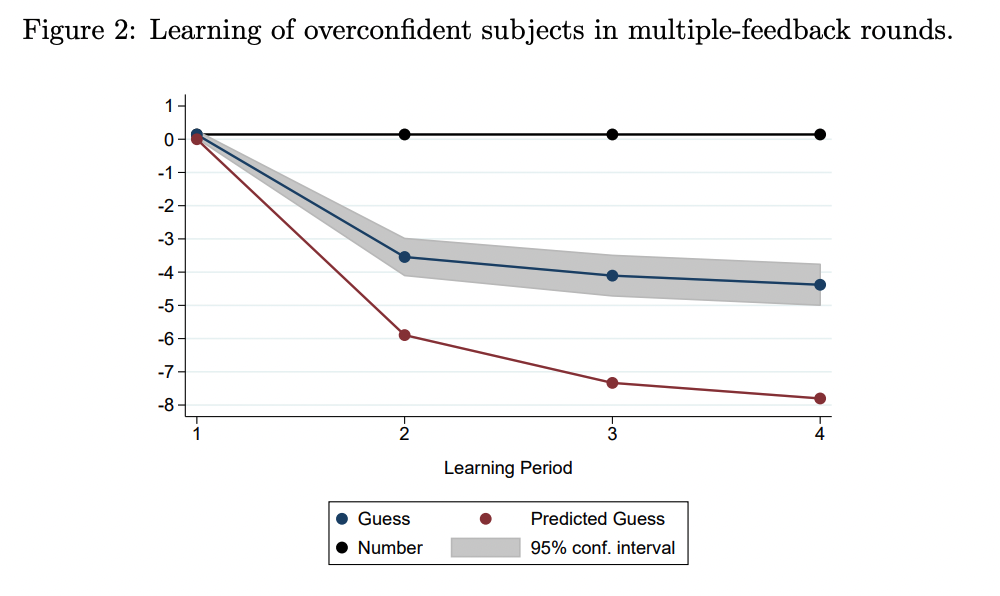
\includegraphics[scale=0.5]{figures/GK_experiment.png}
\end{figure}
    \hyperlink{Other Figures}{\beamerbutton{Other Figures}}

\end{frame}

\begin{frame}{Results}
    Biased updating in the same direction as the theoretical predictions.\\
    \bigskip
    The bias is not as large as the theory predicts.\\
    \bigskip
    Some agents do update their belief of $\theta$ in the right direction.\\
\end{frame}


\begin{frame}{Theory 2: Switchers}
    \Large\textbf{ Robust Misspecified Models and Paradigm Shifts \\}
    (Ba, 2022 JMP)
\end{frame}


\begin{frame}{The Setting}
    Same as HKS but with finite $\Omega$ and finite $A$\\
    \bigskip
    Now the entrepreneur is willing to switch to an alternative level of ability $\theta'$ (assume $\theta' = \theta^*$).\\
    \bigskip
    Instead of updating $P[\theta]$ every period, they perform a Bayesian hypothesis test:\\
    \bigskip
    Adopt model $\theta'$ at time t iff \\
    $$\frac{\ell_t (\theta')}{\ell_t(\theta)}>\alpha\geq1$$

    Where $$\ell_t(\theta) := \sum_{\omega}g_0(\omega)\prod_{\tau=0}^{t-1}\pi^\theta(y_\tau|a_\tau, \omega)$$
  
\end{frame}

\begin{frame}{Results}

    The self-defeating trap is difficult to escape when the entrepreneur is overconfident.\\
    \bigskip
    Underconfident agents escape the trap at a higher rate than overconfident and learn the true parameter.\\
    \bigskip
    Explains why underconfidence is less prevalent in the data.\\
    \bigskip
    Overconfident agents can escape the trap if their prior is not too ``tight'' around a self confirming equilibrium.
  
\end{frame}

\begin{frame}{Theory 3: Motivated Beliefs}
    \Large\textbf{Optimal Expectations}\\
    (Brunnermeier and Parker, 2005)\\
    \bigskip
    \Large\textbf{What to blame? Self-serving attribution bias with
multi-dimensional uncertainty}\\
    (Coutts et al., 2022 wp)
\end{frame}

\begin{frame}{The Setting}
    A fixed effort $e$, $\theta \in \{\theta_H, \theta_L\}$ and $\omega \in \{\omega_H, \omega_L\}$ generate binary signals (success/failure)\\
    \bigskip
    After a success the agent updates their belief about $\theta$ with distortions $\gamma_\theta$ and $\gamma_\omega$, $p_{t+1}(\theta_H|success)$ is given by:\\
    \begin{center}
        \small
        $\frac{\gamma^s_\theta\gamma^s_\omega\pi_t(\theta_H) g_t(\omega_H) q_t(\theta_H, \omega_H) + \gamma^s_\theta\pi_t(\theta_H) g_t(\omega_L) q_t(\theta_H, \omega_L)}{\gamma^s_\theta\gamma^s_\omega\pi_t(\theta_H) g_t(\omega_H) q_t(\theta_H, \omega_H) + \gamma^s_\theta\pi_t(\theta_H) g_t(\omega_L) q_t(\theta_H, \omega_L) + \gamma^s_\omega\pi_t(\theta_L) g_t(\omega_H) q_t(\theta_L, \omega_H) + \pi_t(\theta_L) g_t(\omega_L) q_t(\theta_L, \omega_L)}$\\
    \end{center}
    \bigskip
    with $q_t(\theta, \omega):=Pr[\text{success}|\theta, \omega]$ increasing in $\omega$ and $\theta$
\end{frame}

\begin{frame}{Predictions and Evidence (Coutts et al. 2022)}
    Prediction: Even unbiased agents will overweight $\theta_H$ after a success and end up being biased.\\
    \bigskip
    Experiment: Evidence of biased updating when $\theta$ is ego-relevant.\\
    \bigskip
    The framework does not allow direct comparisons with the other two theoretical predictions.\\
    \bigskip
    It gives an alternative rationalization for the persistence of overconfidence.
    
    
\end{frame}

\begin{frame}{A framework where we can compare}

Finite type space: $\theta \in \{\theta_H, \theta_M, \theta_L\}$\\
\bigskip
Finite state space: $\omega \in \{\omega_H, \omega_M, \omega_L\}$
with $p(\omega_k)=1/3$ \\
\bigskip
Finite action space: $e \in \{e_H, e_M, e_L\}$\\
\bigskip
Binary signal: Success/Failure with $P\left[Success|e, \omega, \theta\right]$ satisfying the assumptions of HKS


\end{frame}

\begin{frame}{The Data Generating Process}
The probability of success is given by:\\
\bigskip
\centering
\begin{tabular}{ c|c|c|c|}
  
  \multicolumn{1}{c}{} & \multicolumn{1}{c}{$\omega_H$} & \multicolumn{1}{c}{$\omega_M$} & \multicolumn{1}{c}{$\omega_L$}\\
  \cline{2-4}
  $e_H$ & 50 & 20 & 2 \\
  \cline{2-4}
  $e_M$ & 45 & 30 & 7 \\
  \cline{2-4}
  $e_L$ & 40 & 25 & 20 \\
  \cline{2-4}
  \multicolumn{1}{c}{} & \multicolumn{1}{c}{} & \multicolumn{1}{c}{$\theta_L$} & \multicolumn{1}{c}{}\\
\end{tabular}
\hspace{.3cm} % adjust this value to set the space between tables
\begin{tabular}{ c|c|c|c|}
  
  \multicolumn{1}{c}{} & \multicolumn{1}{c}{$\omega_H$} & \multicolumn{1}{c}{$\omega_M$} & \multicolumn{1}{c}{$\omega_L$}\\
  \cline{2-4}
  $e_H$ & 80 & 50 & 5 \\
  \cline{2-4}
  $e_M$ & 69 & 65 & 30 \\
  \cline{2-4}
  $e_L$ & 65 & 45 & 40 \\
  \cline{2-4}
  \multicolumn{1}{c}{} & \multicolumn{1}{c}{} & \multicolumn{1}{c}{$\theta_M$} & \multicolumn{1}{c}{}\\
\end{tabular}
\hspace{.3cm} % adjust this value to set the space between tables
\begin{tabular}{ c|c|c|c|}
  
  \multicolumn{1}{c}{} & \multicolumn{1}{c}{$\omega_H$} & \multicolumn{1}{c}{$\omega_M$} & \multicolumn{1}{c}{$\omega_L$}\\
  \cline{2-4}
  $e_H$ & 98 & 65 & 25 \\
  \cline{2-4}
  $e_M$ & 80 & 69 & 35 \\
  \cline{2-4}
  $e_L$ & 75 & 55 & 45 \\
  \cline{2-4}
  \multicolumn{1}{c}{} & \multicolumn{1}{c}{} & \multicolumn{1}{c}{$\theta_H$} & \multicolumn{1}{c}{}\\
\end{tabular}


    
\end{frame}

\begin{frame}{The Data Generating Process}
    \centering
\begin{tabular}{ c|c|c|c|}
  
  \multicolumn{1}{c}{} & \multicolumn{1}{c}{$\omega_H$} & \multicolumn{1}{c}{$\omega_M$} & \multicolumn{1}{c}{$\omega_L$}\\
  \cline{2-4}
  $e_H$ & \cellcolor{blue!25}50 & 20 & 2 \\
  \cline{2-4}
  $e_M$ & 45 & \cellcolor{blue!25}30 & 7 \\
  \cline{2-4}
  $e_L$ & 40 & 25 & \cellcolor{blue!25}20 \\
  \cline{2-4}
  \multicolumn{1}{c}{} & \multicolumn{1}{c}{} & \multicolumn{1}{c}{$\theta_L$} & \multicolumn{1}{c}{}\\
\end{tabular}
\hspace{.3cm} % adjust this value to set the space between tables
\begin{tabular}{ c|c|c|c|}
  
  \multicolumn{1}{c}{} & \multicolumn{1}{c}{$\omega_H$} & \multicolumn{1}{c}{$\omega_M$} & \multicolumn{1}{c}{$\omega_L$}\\
  \cline{2-4}
  $e_H$ & \cellcolor{blue!25}80 & 50 & 5 \\
  \cline{2-4}
  $e_M$ & 69 & \cellcolor{blue!25}65 & 30 \\
  \cline{2-4}
  $e_L$ & 65 & 45 & \cellcolor{blue!25}40 \\
  \cline{2-4}
  \multicolumn{1}{c}{} & \multicolumn{1}{c}{} & \multicolumn{1}{c}{$\theta_M$} & \multicolumn{1}{c}{}\\
\end{tabular}
\hspace{.3cm} % adjust this value to set the space between tables
\begin{tabular}{ c|c|c|c|}
  
  \multicolumn{1}{c}{} & \multicolumn{1}{c}{$\omega_H$} & \multicolumn{1}{c}{$\omega_M$} & \multicolumn{1}{c}{$\omega_L$}\\
  \cline{2-4}
  $e_H$ & \cellcolor{blue!25}98 & 65 & 25 \\
  \cline{2-4}
  $e_M$ & 80 & \cellcolor{blue!25}69 & 35 \\
  \cline{2-4}
  $e_L$ & 75 & 55 & \cellcolor{blue!25}45 \\
  \cline{2-4}
  \multicolumn{1}{c}{} & \multicolumn{1}{c}{} & \multicolumn{1}{c}{$\theta_H$} & \multicolumn{1}{c}{}\\
\end{tabular}
\end{frame}



\begin{frame}{The Data Generating Process}
\begin{center}
\begin{tikzpicture}
  \draw[<-] (1,0) -- (3,0);
  \draw[<-] (5,0) -- (7,0);
  \draw[<-] (9,0) -- (11,0);
\end{tikzpicture}
\end{center}
\\
\bigskip
\centering
\begin{tabular}{ c|c|c|c|}
  
  \multicolumn{1}{c}{} & \multicolumn{1}{c}{$\omega_H$} & \multicolumn{1}{c}{$\omega_M$} & \multicolumn{1}{c}{$\omega_L$}\\
  \cline{2-4}
  $e_H$ & \cellcolor{blue!25}50 & 20 & 2 \\
  \cline{2-4}
  $e_M$ & 45 & \cellcolor{blue!25}30 & 7 \\
  \cline{2-4}
  $e_L$ & 40 & 25 & \cellcolor{blue!25}20 \\
  \cline{2-4}
  \multicolumn{1}{c}{} & \multicolumn{1}{c}{} & \multicolumn{1}{c}{$\theta_L$} & \multicolumn{1}{c}{}\\
\end{tabular}
\hspace{.3cm} % adjust this value to set the space between tables
\begin{tabular}{ c|c|c|c|}
  
  \multicolumn{1}{c}{} & \multicolumn{1}{c}{$\omega_H$} & \multicolumn{1}{c}{$\omega_M$} & \multicolumn{1}{c}{$\omega_L$}\\
  \cline{2-4}
  $e_H$ & \cellcolor{blue!25}80 & 50 & 5 \\
  \cline{2-4}
  $e_M$ & 69 & \cellcolor{blue!25}65 & 30 \\
  \cline{2-4}
  $e_L$ & 65 & 45 & \cellcolor{blue!25}40 \\
  \cline{2-4}
  \multicolumn{1}{c}{} & \multicolumn{1}{c}{} & \multicolumn{1}{c}{$\theta_M$} & \multicolumn{1}{c}{}\\
\end{tabular}
\hspace{.3cm} % adjust this value to set the space between tables
\begin{tabular}{ c|c|c|c|}
  
  \multicolumn{1}{c}{} & \multicolumn{1}{c}{$\omega_H$} & \multicolumn{1}{c}{$\omega_M$} & \multicolumn{1}{c}{$\omega_L$}\\
  \cline{2-4}
  $e_H$ & \cellcolor{blue!25}98 & 65 & 25 \\
  \cline{2-4}
  $e_M$ & 80 & \cellcolor{blue!25}69 & 35 \\
  \cline{2-4}
  $e_L$ & 75 & 55 & \cellcolor{blue!25}45 \\
  \cline{2-4}
  \multicolumn{1}{c}{} & \multicolumn{1}{c}{} & \multicolumn{1}{c}{$\theta_H$} & \multicolumn{1}{c}{}\\
\end{tabular}

\begin{center}
    \resizebox{0.6\linewidth}{!}{\vector(1,0){300}}
  \end{center}
    
\end{frame}

\begin{frame}{A Self-Confirming Equilibrium}

\centering
\begin{tabular}{ c|c|c|c|}
  
  \multicolumn{1}{c}{} & \multicolumn{1}{c}{$\omega_H$} & \multicolumn{1}{c}{$\omega_M$} & \multicolumn{1}{c}{$\omega_L$}\\
  \cline{2-4}
  $e_H$ & \cellcolor[HTML]{b84f79}50 & 20 & 2 \\
  \cline{2-4}
  $e_M$ & 45 & 30 & 7 \\
  \cline{2-4}
  $e_L$ & 40 & 25 & 20 \\
  \cline{2-4}
  \multicolumn{1}{c}{} & \multicolumn{1}{c}{} & \multicolumn{1}{c}{$\theta_L$} & \multicolumn{1}{c}{}\\
\end{tabular}
\hspace{.3cm} % adjust this value to set the space between tables
\begin{tabular}{ c|c|c|c|}
  
  \multicolumn{1}{c}{} & \multicolumn{1}{c}{$\omega_H$} & \multicolumn{1}{c}{$\omega_M$} & \multicolumn{1}{c}{$\omega_L$}\\
  \cline{2-4}
  $e_H$ & 80 & \cellcolor[HTML]{b84f79}50 & 5 \\
  \cline{2-4}
  $e_M$ & 69 &\cellcolor[HTML]{f09ebe}65 & 30 \\
  \cline{2-4}
  $e_L$ & 65 & \cellcolor[HTML]{f09ebe}45 & 40 \\
  \cline{2-4}
  \multicolumn{1}{c}{} & \multicolumn{1}{c}{} & \multicolumn{1}{c}{$\theta_M$} & \multicolumn{1}{c}{}\\
\end{tabular}
\hspace{.3cm} % adjust this value to set the space between tables
\begin{tabular}{ c|c|c|c|}
  
  \multicolumn{1}{c}{} & \multicolumn{1}{c}{$\omega_H$} & \multicolumn{1}{c}{$\omega_M$} & \multicolumn{1}{c}{$\omega_L$}\\
  \cline{2-4}
  $e_H$ & 98 & 65 & 25 \\
  \cline{2-4}
  $e_M$ & 80 & 69 & 35 \\
  \cline{2-4}
  $e_L$ & 75 & 55 & 45 \\
  \cline{2-4}
  \multicolumn{1}{c}{} & \multicolumn{1}{c}{} & \multicolumn{1}{c}{$\theta_H$} & \multicolumn{1}{c}{}\\
\end{tabular}
\end{frame}


\begin{frame}{The Self-Confirming Equilibria}

\centering
\begin{tabular}{ c|c|c|c|}
  
  \multicolumn{1}{c}{} & \multicolumn{1}{c}{$\omega_H$} & \multicolumn{1}{c}{$\omega_M$} & \multicolumn{1}{c}{$\omega_L$}\\
  \cline{2-4}
  $e_H$ & \cellcolor[HTML]{b84f79}50 & 20 & 2 \\
  \cline{2-4}
  $e_M$ & 45 & \cellcolor[HTML]{5f94b8}30 & 7 \\
  \cline{2-4}
  $e_L$ & \cellcolor[HTML]{69a35b}40 & 25 & 20 \\
  \cline{2-4}
  \multicolumn{1}{c}{} & \multicolumn{1}{c}{} & \multicolumn{1}{c}{$\theta_L$} & \multicolumn{1}{c}{}\\
\end{tabular}
\hspace{.3cm} % adjust this value to set the space between tables
\begin{tabular}{ c|c|c|c|}
  
  \multicolumn{1}{c}{} & \multicolumn{1}{c}{$\omega_H$} & \multicolumn{1}{c}{$\omega_M$} & \multicolumn{1}{c}{$\omega_L$}\\
  \cline{2-4}
  $e_H$ & 80 & \cellcolor[HTML]{b84f79}50 & 5 \\
  \cline{2-4}
  $e_M$ & \cellcolor[HTML]{fab143}69 & 65 & \cellcolor[HTML]{5f94b8}30 \\
  \cline{2-4}
  $e_L$ & 65 & \cellcolor[HTML]{9662f0}45 & \cellcolor[HTML]{69a35b}40 \\
  \cline{2-4}
  \multicolumn{1}{c}{} & \multicolumn{1}{c}{} & \multicolumn{1}{c}{$\theta_M$} & \multicolumn{1}{c}{}\\
\end{tabular}
\hspace{.3cm} % adjust this value to set the space between tables
\begin{tabular}{ c|c|c|c|}
  
  \multicolumn{1}{c}{} & \multicolumn{1}{c}{$\omega_H$} & \multicolumn{1}{c}{$\omega_M$} & \multicolumn{1}{c}{$\omega_L$}\\
  \cline{2-4}
  $e_H$ & 98 & 65 & 25 \\
  \cline{2-4}
  $e_M$ & 80 & \cellcolor[HTML]{fab143}69 & 35 \\
  \cline{2-4}
  $e_L$ & 75 & 55 & \cellcolor[HTML]{9662f0}45 \\
  \cline{2-4}
  \multicolumn{1}{c}{} & \multicolumn{1}{c}{} & \multicolumn{1}{c}{$\theta_H$} & \multicolumn{1}{c}{}\\
\end{tabular}
\end{frame}

\begin{frame}{An Example}
\begin{itemize}
    \item True type is $\theta_M$ \\
    \bigskip
    \item True exchange rate is $\omega_M$ $\rightarrow$ The entrepreneur believes it is uniformly distributed\\
    \end{itemize}

    \centering
\begin{tabular}{ c|c|c|c|}
  
  \multicolumn{1}{c}{} & \multicolumn{1}{c}{$\omega_H$} & \multicolumn{1}{c}{$\omega_M$} & \multicolumn{1}{c}{$\omega_L$}\\
  \cline{2-4}
  $e_H$ & 50 & 20 & 2 \\
  \cline{2-4}
  $e_M$ & 45 & 30 & 7 \\
  \cline{2-4}
  $e_L$ & 40 & 25 & 20 \\
  \cline{2-4}
  \multicolumn{1}{c}{} & \multicolumn{1}{c}{} & \multicolumn{1}{c}{$\theta_L$} & \multicolumn{1}{c}{}\\
\end{tabular}
\hspace{.3cm} % adjust this value to set the space between tables
\begin{tabular}{ c|c|c|c|}
  
  \multicolumn{1}{c}{} & \multicolumn{1}{c}{$\omega_H$} & \multicolumn{1}{c}{$\omega_M$} & \multicolumn{1}{c}{$\omega_L$}\\
  \cline{2-4}
  $e_H$ & 80 & \cellcolor{blue!25}50 & 5 \\
  \cline{2-4}
  $e_M$ & 69 & \cellcolor{blue!25}65 & 30 \\
  \cline{2-4}
  $e_L$ & 65 & \cellcolor{blue!25}45 & 40 \\
  \cline{2-4}
  \multicolumn{1}{c}{} & \multicolumn{1}{c}{} & \multicolumn{1}{c}{$\theta_M$} & \multicolumn{1}{c}{}\\
\end{tabular}
\hspace{.3cm} % adjust this value to set the space between tables
\begin{tabular}{ c|c|c|c|}
  
  \multicolumn{1}{c}{} & \multicolumn{1}{c}{$\omega_H$} & \multicolumn{1}{c}{$\omega_M$} & \multicolumn{1}{c}{$\omega_L$}\\
  \cline{2-4}
  $e_H$ & 98 & 65 & 25 \\
  \cline{2-4}
  $e_M$ & 80 & 69 & 35 \\
  \cline{2-4}
  $e_L$ & 75 & 55 & 45 \\
  \cline{2-4}
  \multicolumn{1}{c}{} & \multicolumn{1}{c}{} & \multicolumn{1}{c}{$\theta_H$} & \multicolumn{1}{c}{}\\
\end{tabular}
    
\end{frame}

\begin{frame}{Example: Dogmatic Modeler}
\begin{itemize}
    \item Theory 1: for an entrepreneur who believes he is $\theta_H$
    \end{itemize}
    \bigskip
    \begin{enumerate}
        \item Chooses $e_H$ and is disappointed $\rightarrow$ adjust belief about $\omega$ downward\\
        \bigskip
        \item Eventually chooses $e_M$ and is disappointed as well $\rightarrow$ adjust belief about $\omega$\\
        \bigskip
        \item Eventually chooses $e_L$ and falls into a self-confirming equilibrium
    \end{enumerate}
    
    
\end{frame}

\begin{frame}{Dogmatic Overconfident}
    \begin{figure}
        \centering
        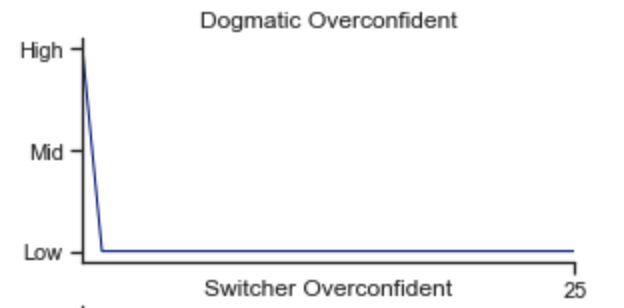
\includegraphics[trim=0 20 0 0, clip]{figures/dogmatic.png}
        \caption{$\theta^*=\theta_M$, $\hat\theta=\theta_H$, $\omega^*=\omega_M$}
    \end{figure}
\end{frame}


\begin{frame}{Example: Likelihood Testing}
\begin{itemize}
    \item Theory 2: for the same initial belief
    \item Keeping track of the likelihood of each $\theta$
    \end{itemize}
    \bigskip
    \begin{enumerate}
        \item Chooses $e_H$ and is disappointed $\rightarrow$ adjust belief about $\omega$ downward\\
        \bigskip
        \item Eventually chooses $e_M$ and is disappointed as well $\rightarrow$ adjust belief about $\omega$\\
        \bigskip
        \item Eventually chooses $e_L$ and falls into a self-confirming equilibrium\\
        \bigskip
        \item At some point, the likelihood of $\theta_M$ becomes much larger than that of $\theta_H$ and the agent updates their belief
    \end{enumerate}
    
    
\end{frame}

\begin{frame}{Switcher Overconfident}
    \begin{figure}
        \centering
        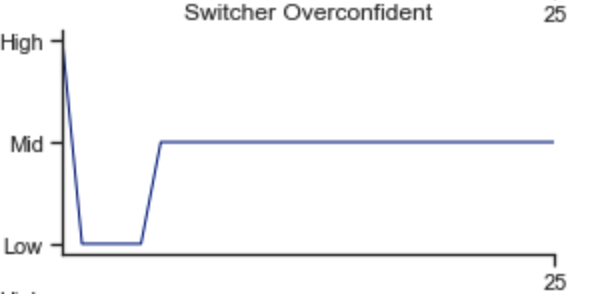
\includegraphics{figures/switch.png}
        \caption{$\theta^*=\theta_M$, $\hat\theta=\theta_H$, $\omega^*=\omega_M$, $\alpha= 1.1$}
    \end{figure}
\end{frame}


\begin{frame}{Example: Self-Serving Beliefs}
\begin{itemize}
    \item Theory 3: Start with a diffused prior over $\theta$
    \end{itemize}
    \bigskip
    \begin{enumerate}
        \item Chooses $e$ that maximizes utility according to priors
        \bigskip
        \item Success $\rightarrow$ overweight $\theta_H$ and underweight $\omega_H$\\
        \item Failure $\rightarrow$ overweight $\omega_L$ underweight $\theta_L$\\
        \bigskip
        \item Belief on $\omega$ deteriorates a lot after failure streaks
        \item Belief on $\theta$ increases a lot after success streaks\\
    \end{enumerate}
    
    
\end{frame}

\begin{frame}{Dogmatic Overconfident}
    \begin{figure}
        \centering
        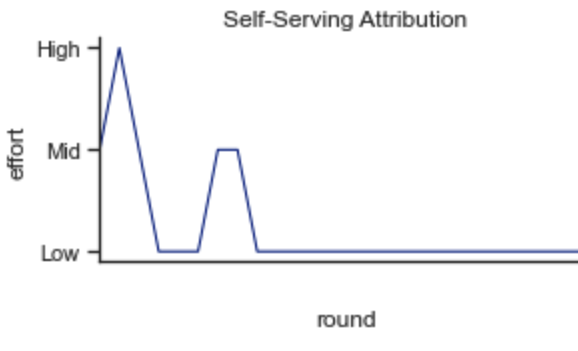
\includegraphics{figures/SS.png}
        \caption{$\gamma^s_\theta=1.2$, $\gamma^s_\omega = .8$}
    \end{figure}
\end{frame}


\begin{frame}{The Simulation}
\label{Figure2}
    \begin{figure}
    \centering
    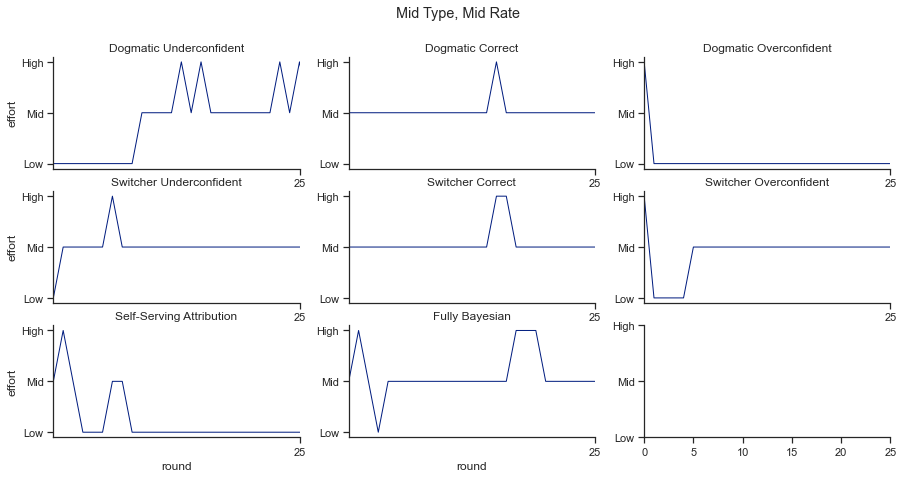
\includegraphics[scale=0.43]{figures/all_1_1.png}
\end{figure}     

\hyperlink{WorstCase}{\beamerreturnbutton{Other Cases}} 

\end{frame}


\begin{frame}{The Experiment:}
Brief Questionnaire: Age, Gender, Nationality, Major\\
\bigskip
Part 1: Set Types\\
\bigskip
\begin{itemize}
    \item Quiz: Answer as many questions as you can in 2 minutes:\\
    \begin{itemize}
        \item Math, Verbal, Pop-Culture, Science, Us Geography, Sports and Videogames\\
    \end{itemize}
    \bigskip
    \item How many questions do you think you answered correctly in each quiz?\\
    \begin{itemize}
        \item[o] Bin1, Bin2, Bin3
    \end{itemize}
\end{itemize}

\end{frame}


\begin{frame}{The Experiment: Ego-relevant condition}
Belief updating and effort choice (One topic at a time)\\
\bigskip
\begin{itemize}
    \item Choose an effort
    \item Receive a signal realization
\end{itemize}
\bigskip
25 rounds per topic

\end{frame}

\begin{frame}{Eliciting Beliefs?}
\begin{itemize}
    \item $E[\omega]$ is revealed by their choice of effort\\
    \bigskip
    \item Eliciting beliefs for $\theta$ can incentivize learning in a way that is not consistent with the model\\
    \bigskip
\end{itemize}

Allow them to see the success rate matrix for only one type. 
\begin{itemize}
    \item Track the matrices they choose to see in each round
\end{itemize}



\end{frame}

\begin{frame}{The Experiment: Ego-irrelevant condition}

Observe the characteristics of a participant. 
\begin{itemize}
    \item ``What score do you think this participant got in the (topic) quiz?'' 
    \item Bin1, Bin2, Bin3 
\end{itemize}

Belief updating and effort choice\\
\bigskip
\begin{itemize}
    \item Choose an effort
    \item Receive a signal realization
    \begin{itemize}
        \item[o] The DGP is that of the observed participant
    \end{itemize}
\end{itemize}
\bigskip
25 rounds (per topic/participant)

\end{frame}

\begin{frame}{Conclusion}
What I hope to get from this design:\\
\bigskip
    \begin{itemize}
        \item A classification of subjects into one of the models based on their behavior\\
        \bigskip
        \item If subjects are switchers: what is the switching threshold $\alpha$\\
        \bigskip
        \item Insight into the role of ego-relevant parameters in belief misspecification
    \end{itemize}
\end{frame}

\begin{frame}{The end}
    \large\textbf{Thank you!}
\end{frame}

\begin{frame}{Götte and Kozakiewicz (2022) }
\label{Other Figures}
    \begin{figure}
    \centering
    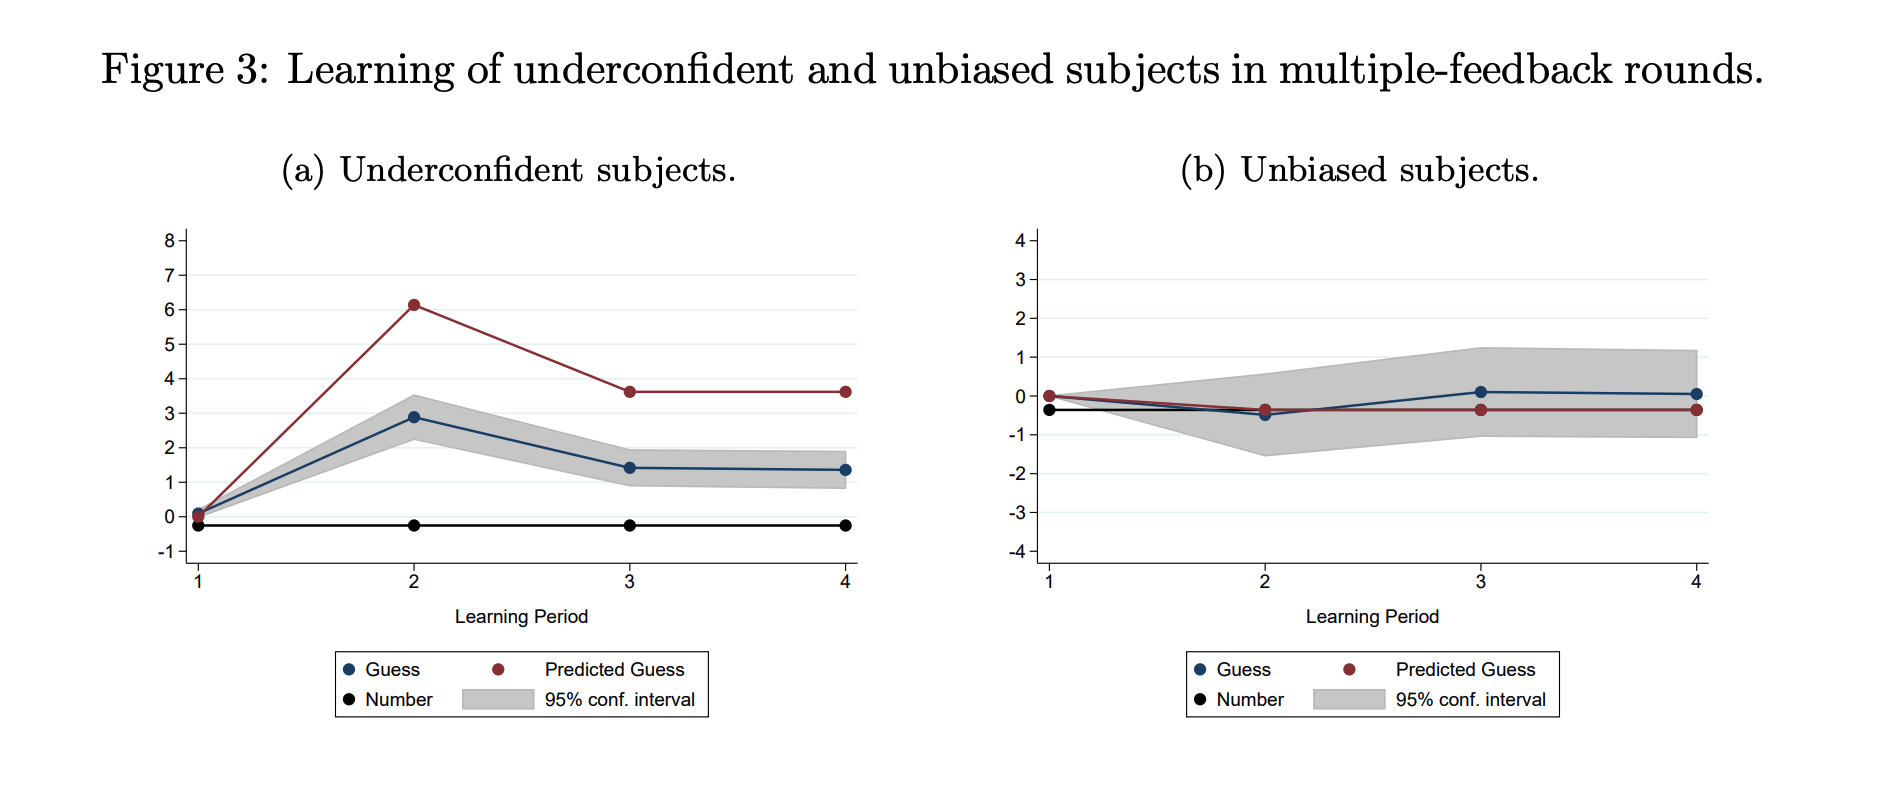
\includegraphics[scale=0.45]{figures/GK_under-unbiased.png}
\end{figure}


\hyperlink{Figure1}{\beamerreturnbutton{Back}}       

\end{frame}

\begin{frame}{A Bad Case}
\label{WorstCase}
    \begin{figure}
    \centering
    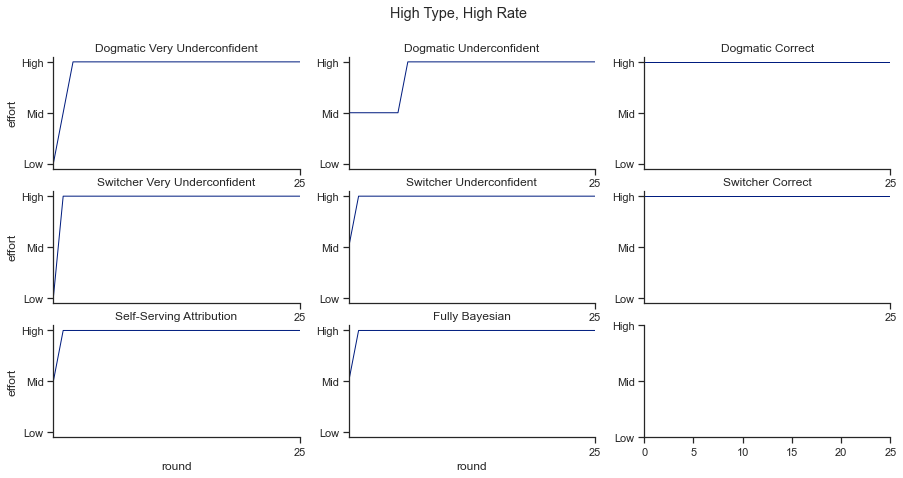
\includegraphics[scale=0.4]{figures/all_2_2.png}
\end{figure}


\hyperlink{Figure2}{\beamerreturnbutton{Back}}       

\end{frame}

\end{document}

